% Windows: протестировано для MikTeX+TeXworks в режиме pdfLatex.
%
% Linux:
% Для получения pdf используйте команду  pdflatex rfa_2021.tex.
% Команда latex rfa_2021.tex выведет сообщение об ошибке.
%
\NeedsTeXFormat{LaTeX2e}
\documentclass[10pt,a4paper]{book}
\usepackage{NumMet_2023}
%--- Здесь можно вставить необходимые стили ---
% \usepackage{...}
%
%--- Здесь можно добавить свои команды --------
% \newcommand{}
\newcommand{\ceq}{\mathrel{\vcenter{\hbox{:=}}}}
%----------------------------------------------
\selectlanguage{russian}
\begin{document}
%===========================  ШАПКА СТАТЬИ =================================
\Article{Сходимость алгоритма липшицевой глобальной\break
    оптимизации для частично определенной функции}
    {Convergence of the Lipschitz Global Optimization Algorithm\break
    for a Partially Defined Function}
    
\Abstract{В статье обсуждается проблема нахождения глобального минимума липшецевой функции, которая может быть частично определена в области поиска. Такое явление возможно в силу особенностей оптимизируемого объекта и метода моделирования (например, численная нестабильность). В некоторых случаях эти подобласти известны, но в большинстве случаев информация о них отсутствует. В статье изложено описание модификации алгоритма глобального поиска для решения такого класса задач. Даны теоретические обоснования сходимости алгоритма.}
    {The paper discusses the problem of finding the global minimum of a Lipschitz function that may be partially defined in the search domain. This phenomenon is possible due to the nature of the optimized object and of the simulation method (for example, numerical instability). In some cases, these subareas are known, but in most cases the information about them is missing. The paper provides a modification the global search algorithm for solving this class of problems. Theoretical justifications for the convergence of the algorithm are given. The results of numerical experiments are presented.}

\Keywords{липшецева глобальная оптимизация, 
        многоэкстремальные функции, 
        частично определенные функции,
        условия сходимости.}
        {lipschitz global optimization, 
        multiextremal functions, 
        partially defined functions,
        convergence conditions.}

\Acknowledgements{Работа выполнена при поддержке Министерства науки и высшего образования Российской Федерации (проект \No~FSWR-2023-0034) и Научно-образовательного математического центра ``Математика для технологий будущего''.}
    {The work was supported by the Ministry of Science and Higher Education of the Russian Federation (project no.~FSWR-2023-0034) and by the Research and Education Mathematical Center ``Mathematics for Future Technologies''.}

\Citation{Усова~М.А., Баркалов~К.А.
    Сходимость алгоритма липшицевой глобальной оптимизации
    для частично определенной функции~//
    Вычислительные методы и программирование. 2024.
    \textbf{??}, \No~?. \pageref*{firstPage}--\pageref*{LastPage}.  
    doi 10.26089/NumMet.v??r???.}
    {M.~A.~Usova, K.~A.~Barkalov
    ``Convergence of the Lipschitz Global Optimization Algorithm
    for a Partially Defined Function'',
    Numerical Methods and Programming. \textbf{??} (?), 
    \pageref*{firstPage}--\pageref*{LastPage} (2024).
    doi~10.26089/NumMet.v??r???.}


\UDC{<указывает автор>}
\DOI{10.26089/NumMet.v??r???}% заполняет редакция
\VOL{??}{?}
\YEAR{2024}
\Received{16 июня 2024 г.}{June 16, 2024}
\Accepted{13 октября 2024 г.}{October 13, 2024}


\Author{М.~А.~Усова}{M.~A.~Usova}
\FullName{Марина~Андреевна~Усова}{Marina~A.~Usova}
\Institution{Национальный исследовательский Нижегородский государственный университет им.~Н.~И.~Лобачевского}
{National Research Lobachevsky State University of Nizhni Novgorod}
\Address{пр.Гагарина, 23}{Gagarina Prospekt, 23}
\Postcode{603022}
\City{Нижний Новгород}{Nizhni Novgorod}
\CountryOfResidence{Российская Федерация}{Russia}
%\Position{мл. науч. сотр.}{Assistant Research Fellow}
\Orcid{0000-0002-0722-6884}
\Email{usova@itmm.unn.ru}

\Author{К.~А.~Баркалов}{K.~A.~Barkalov}
\FullName{Константин~Александрович~Баркалов}{Konstantin~A.~Barkalov}
\Institution{Национальный исследовательский Нижегородский государственный университет им.~Н.~И.~Лобачевского}
{National Research Lobachevsky State University of Nizhni Novgorod}
\Address{пр.Гагарина, 23}{Gagarina Prospekt, 23}
\Postcode{603022}
\City{Нижний Новгород}{Nizhni Novgorod}
\CountryOfResidence{Российская Федерация}{Russia}
\AcademicDegree{д-р техн. наук.}{D.Eng.}
%\Position{мл. науч. сотр.}{Assistant Research Fellow}
\Orcid{0000-0001-5273-2471}
\Email{konstantin.barkalov@itmm.unn.ru}

\MakeArticleHeader
%========================= КОНЕЦ ШАПКИ СТАТЬИ ==============================

\pagebreak

\section{Введение}

Процесс выбора оптимальных значений параметров в различных приложениях часто подразумевает решение задачи \textit{глобальной (многоэкстремальной) оптимизации}. В таких задачах для целевой функции обычно не известно аналитическое выражение; ее значения вычисляются посредством численного моделирования оптимизируемого объекта (т.е. функция задана как «черный ящик»). При этом даже одно вычисление значения функции в некоторой точке области поиска (данную процедуру будем называть \textit{поисковым испытанием}) может потребовать существенных ресурсов. Типичными примерами задач глобальной оптимизации с функциями вида <<черный ящик>> являются задачи идентификации параметров математических моделей по экспериментальным данным [\colorbox[rgb]{1,1,0}{ссылки}].


%Широко распространенными математическими моделями процесса выбора оптимальных значений параметров в различных приложениях являются задачи глобальной оптимизации. В таких задачах целевая функция обычно не задана аналитическим выражением, ее значения вычисляются программно (т.е. функция задана как «черный ящик»). При этом даже одно вычисление значения функции в некоторой точке области поиска (в дальнейшем этот процесс будем называть \textit{поисковым испытанием}) может потребовать существенного времени.Типичными примерами задач глобальной оптимизации с функциями вида «черный ящик» являются задачи идентификации параметров математических моделей по экспериментальным данным [ссылки].

Задачи глобальной оптимизации относятся к числу наиболее сложных оптимизационных задач, т.к. отыскание абсолютного экстремума требует вычисления значений функции в узлах некоторой адаптивной сетки в области поиска. 
Построение достоверных оценок глобального оптимума в многоэкстремальных задачах принципиально основано на использовании априорной информации, позволяющей связать возможные значения целевой функции с известными значениями в точках проведенных поисковых испытаний.
Весьма часто такая информация представляется в виде предположения, что целевая функция $\phi(y)$ удовлетворяет в области поиска условию Липшица, причем константа Липшица $L$, характеризующая скорость изменения функции, является неизвестной. В прикладных задачах это предположение соответствует условию ограниченности изменения характеристик оптимизируемого объекта при ограниченном изменении его параметров. 

Для решения задач липшицевой глобальной оптимизации предложен ряд эффективных алгоритмов 
[\ref{rfa:rulit:Grishagin2016_2},\ref{rfa:rulit:Jones2021},\ref{rfa:rulit:PaulaviciusZilinskas2014},\ref{rfa:rulit:Birect2020},\ref{rfa:rulit:Sergeyev2017}]. Указанные методы относятся к классу детерминированных и превосходят (в терминах количества испытаний, требующегося для корректного решения задачи) широко распространенные метаэвристические алгоритмы (см. результаты сравнения в [\ref{rfa:rulit:Sovrasov2019},\ref{rfa:rulit:Sergeyev2018}]).
Данная работа продолжает развитие одного из известных детерминированных алгоритмов решения задач липшицевой глобальной оптимизации -- алгоритма глобального поиска (АГП) [\ref{rfa:rulit:Sergeyev2013},\ref{rfa:rulit:Strongin2000}]. В рамках рассматриваемого подхода решение многомерных задач сводится к решению эквивалентных им задач одномерной оптимизации. Соответствующая редукция основана на использовании кривых Пеано-Гильберта, однозначно отображающих единичный отрезок вещественной оси на многомерную область поиска. 
 
%Отметим, что для оптимизации сложных объектов реального мира естественным является использование при расчетах сложных математических моделей, что, как следствие, существенно увеличивает трудоемкость поиска оптимума. За последние десятилетия специалистами в области оптимизации и параллельных вычислений было предложено множество способов снижения вычислительной сложности и ускорения используемых алгоритмов, связанных как с решением возникающих оптимизационных задач [\ref{rfa:rulit:Kvasov2013},\ref{rfa:rulit:Sergeyev2020}], так и с численным анализом исходных моделей [\ref{rfa:rulit:Dongarra2022},\ref{rfa:rulit:Duwe2020}].
В последнее время при решении прикладных оптимизационных задач актуальной становится проблема численной нестабильности исследуемых моделей в некоторых (заранее не известных) подобластях области изменения параметров.
В таких подобластях невозможно корректно провести численное моделирование и вычислить значение целевого критерия.
Например, подобные эффекты возникают при численном моделировании обледенения лопаток вентилятора газотурбинного двигателя [\ref{rfa:rulit:Modorskii}].
Данное свойство можно интерпретировать как наличие в оптимизационной задаче скрытых ограничений [\ref{rfa:rulit:Stripinis2021}], либо как существование  заранее неизвестных областей неопределенности целевой функции [\ref{rfa:rulit:Audet2022}], либо как частичную вычислимость целевой функции в области поиска [\ref{rfa:rulit:Candelieri2019},\ref{rfa:rulit:Strongin2020}]. В такой постановке задача оптимизации существенно усложняется, т.к. область допустимых сочетаний параметров является заранее неопределенной. Новое предложение, исследуемое в данной статье, связано с модификацией правил алгоритма глобального поиска для корректного решения задач, в которых целевая функция может быть определена не во всей области поиска.

Статья имеет следующую структуру. Первый раздел содержит постановку задачи и описание используемого способа редукции размерности. Вычислительные правила модифицированного алгоритма глобального поиска, обеспечивающего работу с частично определенными целевыми функциями, приведены во втором разделе. В третьем разделе доказаны теоретические утверждения о сходимости предложенного алгоритма. В четвертом разделе приведено описание генератора, порождающего тестовые задачи с не всюду определенной целевой функцией. Использование генератора задач позволяет оценить эффективность предложенного алгоритма путем численного решения большой серии задач, в том числе -- провести его сравнение с известными методами глобальной оптимизации. В заключительном разделе обсуждаются полученные результаты и формулируются направления дальнейших исследований.


\section{Постановка задачи}

В общем виде задача глобальной оптимизации может быть сформулирована следующим образом:
\begin{equation}\label{eq1} 
\phi^*=\phi(y^* )=\min_{y \in D} \phi(y), D=\left\{ y \in R^N: a_i \leq y_i \leq b_i, \; 1 \leq i \leq N \right\},
\end{equation}
где $y=(y_1,y_2,...,y_N)$ -- вектор варьируемых параметров, $D$ -- $N$-мерный гиперкуб, $N$ –- размерность решаемой задачи.

Будем предполагать, что целевая функция $\phi (y)$:
\begin{enumerate}
\item{является многоэкстремальной и, возможно, недифференцируемой;}
\item {задана как <<черный ящик>> -- в виде некоторой вычислительной процедуры, на вход которой подается аргумент, а выходом является соответствующее значение функции;}
\item{является вычислительно трудоемкой, т.е. проведение одного поискового испытания может потребовать существенного времени;}
\item{определена и вычислима только в некоторой заранее неизвестной подобласти $Q \subseteq D$ положительного объема.}
\end{enumerate}

%методов липшицевой оптимизации [\ref{rfa:rulit:PaulaviciusZilinskas2014},\ref{rfa:rulit:Sergeyev2017}].
%На случай решения задач с невсюду вычислимой целевой функцией нами была разработана модификация алгоритма глобального поиска (АГП-Н) [\ref{rfa:rulit:Usova2024}].

Подобласть $Q \subseteq D$ будем называть \textit{областью вычислимости} функции $\phi (y)$. 
Соответственно, подобласть $I = D \backslash Q$ будем называть \textit{областью невычислимости} функции $\phi (y)$.
Отметим, что исходя из опыта решения прикладных оптимизационных задач [\ref{rfa:rulit:Barkalov2022},\ref{rfa:rulit:Gubaydullin2022}], суммарный объем области невычислимости $I$ составляет небольшую долю объема области поиска $D$.

Предположение 4 делает невозможными использование базового АГП [\ref{rfa:rulit:Strongin2000}] или его параллельных вариантов [\colorbox[rgb]{1,1,0.6}{ссылки}] для решения задачи (\ref{eq1}).
Чтобы преодолеть это ограничение, будем предполагать, что существует функция $\Phi (y)$, вычислимая во всей области $D$ и удовлетворяющая условию Липшица
\begin{equation}\label{eq3} 
| \Phi (y')-\Phi (y'') | \leq L \| y'-y'' \|, \; y',y'' \in D,
\end{equation}
причем $\phi (y) = \Phi (y), y \in Q$. Функцию $\Phi (y)$ будем называть \textit{липшицевым продолжением} $\phi (y)$ на область $D$. 
Существование функции $\Phi (y)$ позволяет разработать модифицированный алгоритм глобального поиска для решения задач с частично вычислимыми функциями, детальное описание которого приведено в разделе \ref{sec:algorithm}. 

\section{Редукция размерности}\label{sec:reduction}

Многие методы липшицевой глобальной оптимизации для решения многомерных задач используют идею редукции размерности. Указанная редукция может быть основана, например, на построении диагональных кривых [\ref{rfa:rulit:Sergeyev2017}], схеме вложенной оптимизации [\ref{rfa:rulit:Grishagin2016_2}], симплексном разбиении области поиска [\ref{rfa:rulit:PaulaviciusZilinskas2014}].
В нашей работе для редукции размерности используются кривые Пеано-Гильберта $y(x)$, однозначно отображающие отрезок вещественной оси  $[0,1]$ на $N$-мерный единичный гиперкуб
\begin{equation}\label{eq2_} 
D=\left\{ y \in R^N: -2^{-1} \leq y_i \leq 2^{-1}, 1 \leq i \leq N \right\} = \left\{ y(x): 0 \leq x \leq 1 \right\}.
\end{equation}
С их помощью исходную задачу (\ref{eq1}) можно свести к задаче 
\begin{equation}\label{eq2} 
f^*(x)=\phi(y(x^* ))=\min_{x \in [0,1]} \left\{ \phi(y(x)) \right\}
\end{equation}
и применить для ее решения эффективные алгоритмы одномерной оптимизации. 

Отметим, что кривая Пеано-Гильберта определяется как предельный объект, поэтому на практике можно использовать лишь ее аппроксимацию (\textit{развертку}) $y_m(x)$, приближающую истинную кривую $y(x)$ с точностью $2^{-m}$ (целое число $m \geq 1$ является параметром построения развертки). Различные способы численного построения разверток рассмотрены в [\ref{rfa:rulit:Strongin2000}].

Также известно, что схема редукции размерности с использованием разверток сопоставляет многомерной липшицевой функции $\phi(y)$ одномерную функцию $f(x)$, удовлетворяющую условию Гёльдера
\begin{equation}\label{eq4} 
| f(x')-f(x'') | \leq H \rho(x',x''), \; x',x'' \in [0,1],
\end{equation}
где $\rho(x',x'') =  |x' - x''|^{1/N}$ -- метрика Гёльдера, $N$ -- размерность исходной многомерной задачи, а коэффициент $H$ связан с константой Липшица $L$ соотношением $H \leq 2L\sqrt {N+3}$ [\ref{rfa:rulit:Strongin2000}].


\section{Алгоритм решения задач с частично определенной целевой функцией}\label{sec:algorithm}

Предлагаемый алгоритм представляет собой модификацию алгоритма глобального поиска (АГП) и ориентирован на решение задач, в которых целевая функция определена и вычислима только в области $Q \subseteq D$, причем область $Q$ является априори неизвестной. В случае всюду вычислимой целевой функции, т.к. когда $Q=D$, результаты работы нового алгоритма должны соответствовать исходному АГП. Изменения вычислительных правил алгоритма касаются только учета и обработки результатов испытаний, полученных в точках из области невычислимости $I$. 

Отметим, что в редуцированной одномерной задаче (\ref{eq2}) поисковое испытание в точке $x' \in [0,1]$ предполагает сначала построение образа $y' = y(x') \in D$, и лишь затем -- вычисление значения $z'=\phi(y')$. Результатом испытания будет являться набор $(x',y',z')$, причем значение $z'$ будет являться неопределенным, если $y' \in I$. Для исключения обработки неопределенных значений в алгоритме вводится понятие \textit{индекса} точки испытания (см. Правило 1 ниже).

Приведем подробное описание нового алгоритма, на который будем ссылаться как на Алгоритм Глобального Поиска для задач с Не всюду вычислимой целевой функцией, АГП-Н.

\subsection{Вычислительная схема алгоритма}

Первые два испытания проводятся в граничных точках $x^0=0$ и $x^0=1$.
Выбор точки $x^{k+1}, k \geq 1$ очередного $(k+1)$-го испытания осуществляется в соответствии со следующими правилами.

\textit{Правило 1.} Перенумеровать (нижним индексом) точки $x^i, 0 \leq i \leq k$ предшествующих испытаний в порядке возрастания значений координаты, то есть
\begin{equation}\label{eq5} 
0=x_0 < x_1 < ... < x_i < ... < x_{k}=1
\end{equation}
и сопоставить каждой точке значение $z_i=f(x_i)$ и индекс $v_i=v(x_i)$, определяемый по правилу
\begin{equation}\label{eq6} 
v_i=v(x_i)=
  \begin{cases}
    0, & {\quad y(x_i) \in I },\\
    1, & {\quad y(x_i) \in Q}.
  \end{cases}
\end{equation}
%ссылка на множества Q и I.

\textit{Правило 2.} Вычислить величину
\begin{equation}\label{eq7} 
\mu = \max\left\{ \frac{|z_i-z_{i-1}|}{\Delta _i},\quad v(x_{i-1})=v(x_i)=1, \quad 1 \leq i \leq k  \right\},\quad \Delta _i= (x_i-x_{i-1})^{1/N}.
\end{equation}
Если $\mu=0$, то положить $\mu=1$.

\textit{Правило 3.} Определить текущее минимальное значение целевой функции
\begin{equation}\label{eq8} 
z^*= \min \left\{ z_i: v(x_i)=1, 0 \leq i \leq k \right\}.
\end{equation}

\textit{Правило 4.} Для каждого интервала $(x_{i-1},x_i),1 \leq i \leq k$, вычислить значение $R(i)$, называемое \textit{характеристикой} интервала, согласно выражению
\begin{equation}\label{eq9} 
R(i)=
  \begin{cases}
    {(1-\frac{1}{r})}^2 \Delta _i,& {\quad v(x_i)=v(x_{i-1})=0,} \\
    \Delta _i+\frac {{(z_i-z_{i-1})}^2}{{(r \mu)}^2 \Delta _i} - 2 \frac {z_i+z_{i-1}-2z^*}{r \mu}, & {\quad  v(x_i)=v(x_{i-1})=1},\\
    2 \Delta _i-4 \frac {(z_i-z^*)}{r \mu}, & {\quad v(x_{i-1})=0, v(x_i)=1},\\
    2 \Delta _i-4 \frac {(z_{i-1}-z^*)}{r \mu}, & {\quad  v(x_{i-1})=1, v(x_i)=0,}
  \end{cases}
\end{equation}
где $r>1$ -- параметр метода.
\textit{Правило 5.} Определить интервал $(x_{t-1},x_t)$ с максимальным значением характеристики:
\[
R(t)= \max\{R(i): \; 1 \leq i \leq k\}.
\]
Если максимальную характеристику имеют несколько интервалов, выбрать интервал
%с большим количеством вычислимых точек - это можно формализовать как интеврал с наибольшей суммой индексов граничных точек
с минимальным номером.

\textit{Правило 6.} Если $v(x_i)=v(x_{i-1})=1$, то провести очередное испытание в точке 
\begin{equation}\label{eq11} 
x^{k+1}= \frac {x_t+x_{t-1}}{2} -  \text{sign} {(z_t-z_{t-1})} \frac{1}{2r} \left[\frac {{|z_t-z_{t-1}|}}{\mu} \right]^N.
\end{equation}
В противном случае провести очередное испытание в серединной точке интервала $(x_{t-1},x_t)$, т.е.
\begin{equation}\label{eq10} 
x^{k+1}=\frac {x_t+x_{t-1}}{2}.
\end{equation}

\textit{Условие остановки.} Поиск завершается при выполнении условия 
\[
\Delta _t = (x_t-x_{t-1})^{1/N} \leq \varepsilon,
\]
где $t$ из Правила 5, а $\varepsilon>0$ -- параметр алгоритма (точность поиска).

\subsection{Условия сходимости и оценка эффективности}

Различные варианты алгоритмов для решения задач липшицевой оптимизации и соответствующая теория сходимости представлены в работах [\ref{rfa:rulit:Sergeyev2013},\ref{rfa:rulit:Strongin2000}]. Приведём формулировку теоремы сходимости для АГП.

%А нужна ли здесь формулировка теоремы о сходимости АГП? Можно только сослаться на нее
\textbf{Теорема (о сходимости АГП)}. Пусть $\overline{y}=y(\overline{x})$ есть предельная точка последовательности испытаний $\{y^k\}=\{y(x^k)\}, \{x^k\} \subset [0,1]$, порождаемой АГП при минимизации липшицевой с константой $L$ функции $\phi(y), y = y(x) \in D$. Тогда: 

\begin{enumerate}
\item
если у последовательности $\{y^k\}$ одновременно с $\overline{y}$ существует другая предельная точка $y'$, то  $\phi(\overline{y}) = \phi(y')$.
\item
для любого $k \geq 0$ выполняется неравенство $z^k = \phi(y^k) \geq \phi(\overline{y})$
\item
если на некотором шаге поиска выполнено условие 
\[
r\mu > 2^{3-1/N}L\sqrt{N+3},
\]
то любая точка глобального минимума $y^*$ является предельной точкой последовательности $\{y^k\}$ и любая точка $\overline{y}$ является точкой глобального минимума функции $\phi(y)$.
\end{enumerate}

\textbf{Замечание}. Теорема соответствует случаю пустой области невычислимости целевой функции, т.е. $I = \emptyset$ и $Q = D$.

%лемма использует утверждение о том, что R(i)>0, т.е. ее нельзя доказывать раньше теоремы, только внутри нее
\textbf{Лемма} (о попадании испытаний в область вычислимости). Пусть $\{y^k\}=\{y(x^k)\}$ -- последовательность точек испытаний, порождаемая алгоритмом АГП-Н при минимизации частично определенной в области $D$ фукнции $\phi(y)$. Тогда существует номер $h \geq 0$ такой, что точка $y^h = y(x^h)$ принадлежит области вычислимости, т.е. $y^h \in Q$ и $v(x^h) = 1$.

\textbf{Доказательство}. Пусть $y' \in Q$ -- внутренняя точка множества $Q$, а $x' \in [0,1]$ -- ее прообраз на отрезке $[0,1]$, т.е. $y' = y(x')$. Тогда существует такой отрезок $[\alpha, \beta] \subset [0, 1]$, содержащий точку $x'$, что для любой точки $x \in [\alpha, \beta]$ ее образ $y(x)$ попадает в область вычислимости $Q$, т.е. $y(x) \in Q$ (Рис. \ref{fig_1}). 

\begin{figure}[h]
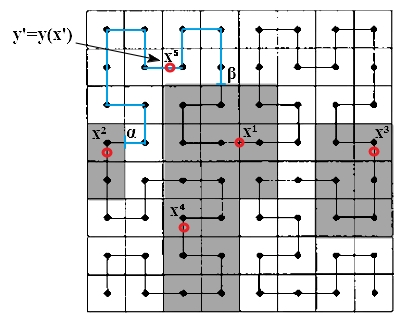
\includegraphics[width=200pt]{pic/fig_1.jpg}
\caption{Существование вычислимого отрезка на кривой Пеано} \label{fig_1}
\end{figure}

Значит на каждом шаге поиска $k \geq 1$ существует некоторый интервал $(x_{j-1}, x_{j})$ такой, что $x' \in (x_{j-1}, x_{j})$. Если $y(x_{j-1})$ или $y(x_{j})$ принадлежат области $Q$, то $v(x_{j-1}) = 1$ или $v(x_j) = 1$ и всё доказано.

Иначе, $R(j)=(1-\frac{1}{r})^2\Delta_j>0$ и в этот интервал попадёт точка одного из следующих испытаний. При $k \to \infty$ алгоритм будет порождать последовательность интервалов, сходящихся к $x'$, а значит через некоторое количество итераций $h$ граница одного из интервалов попадёт в $[\alpha, \beta]$ и $v(x_{j+h-1}) = 1$ или $v(x_{j+h}) = 1$, что доказывает утверждение.

Установим условия сходимости для АГП-Н и покажем, что расширение алгоритма вычисления характеристики не рождает предельных точек другого типа по сравнению с предельными точками классического АГП.
%, кроме предельных точек областей невычислимости.

\textbf{Теорема (о сходимости АГП-Н)}. Пусть $\overline{y}=y(\overline{x})$ есть предельная точка последовательности испытаний $\{y^k\}=\{y(x^k)\}, \{x^k\} \subset [0,1]$, порождаемой АГП-Н при минимизации функции $\phi(y), y \in D$, для которой выполнены следующие условия:
\begin{enumerate}
\item{$\phi(y)$ определена и вычислима в области $Q = D \backslash I$ положительного объёма, где $I$ -- область невычислимости;}
\item{$\phi(y)$ допускает липшицево с константой $L$ продолжение $\Phi(y)$ на область $D$, т.е.
\[
\phi(y(x))=\Phi(y(x)), y(x) \in Q.
\]
}
\end{enumerate}
Тогда если на некотором шаге поиска выполнено условие
\[
r\mu > 2^{3-1/N}L\sqrt{N+3},
\]
то любая точка глобального минимума $y^* \in Q$ является предельной точкой последовательности $\{y^k\}$ и любая точка $\overline{y}$ является либо точкой глобального минимума функции $\phi(y), y \in Q$, либо принадлежит области невычислимости $\overline{y} \in I$.

\textbf{Доказательство}. Во-первых, докажем, что для любой предельной точки $\overline{y}=y(\overline{x}), \overline{x} \in [0,1]$ существует бесконечная последовательность вложенных интервалов, соответсвующих упорядоченным по возрастанию номерам итераций $k_i$, $\{(x_{t-1}, x_t)\}, t = t(k_i), i = 1, 2, ...$, удовлетворяющая условиям:
\[
\lim_{t \to \infty}{\Delta_t} = 0,
\]
\[
\overline{x}=\bigcap_{i = 1}^{\infty}{(x_{t-1}, x_t)},
\]
\[
R(t(k_i))>0, i = 1, 2, ... ,
\]
\[
\lim_{i \to \infty}{R(t(k_i))} = 0,
\]
где $\Delta_t = (x_t - x_{t-1})^{1/N}$, $R(t)$ и $t$ -- из Правила 5 раздела 3.1.

Так как $\overline{x}$ -- предельная точка, то существует последовательность номеров итераций ${k_i}, i = 1, 2, ... $, для которой $x^{k_i+1} \in (x_{t-1}, x_{t})$ и $\overline{x} \in (x_{t-1}, x_{t})$, $t = t(k_i)$, т.е. в интервал, содержащий предельную точку $\overline{x}$, попадает точка очередного испытания $x^{k_{i}+1}$. Из правил вычисления новой точки (\ref{eq10})--(\ref{eq11}), а также оценки (\ref{eq7}) получаем
оценку для максимальной длины очередного поискового интервала
%\[
%x_t-x^{k_i+1} \leq \frac{x_t-x_{t-1}}{2} + \text{sign}(z_t-z_{t-1})\frac{1}{2r}\Delta_t^N \leq \frac{r + 1}{2r}(x_t-x_{t-1}),
%\]
%аналогично для $x^{k_i+1} - x_{t-1}$, тогда справедлива оценка
\[
\max\{x_t-x^{k_i+1},x^{k_i+1} - x_{t-1}\} \leq \gamma(x_t - x_{t - 1}),
\]
где коэффициент $\gamma = \frac{r+1}{2r} < 1$. Отсюда следует, что $\Delta_t \to 0$ при $i \to \infty$ и $\overline{x}=\bigcap_{i = 1}^{\infty}{(x_{t-1}, x_t)}$.

%В предположении, что на каждом шаге $k \geq 1$ существует некоторый интервал $(x_{j-1}, 
Предположим, что на каждом шаге $k \geq h$ существует некоторый интервал $(x_{j-1}, x_{j})$, в одной из точек которого достигается текущее минимальное значение $z^*$, т.е. $z^* = z_j$ или $z^* = z_{j-1}$. Тогда справедливо соотношение $z_j + z_{j-1}-2z^* = |z_j-z_{j-1}| = \mu_j \Delta_j \leq \mu \Delta_j$ и, если обе граничные точки вычислимы $v(x_{j-1}) = v(x_j) = 1$, то из (\ref{eq9}) следует
\[
R(j) = \Delta_j + \frac{(\mu_j \Delta_j)^2}{(r\mu)^2 \Delta_j}-2\frac{\mu_j \Delta_j}{r\mu} = (\Delta_j-\frac{\mu_j\Delta_j}{r\mu})^2 \geq (1-1/r)^2 \Delta_j > 0,
\]
а если $v(x_{j-1}) \neq v(x_j)$, то $R(j)=2\Delta_j>0$. Таким образом, на каждом шаге поиска $k \geq h$ существует интервал со сторого положительной характеристикой. Значит и характеристики лучших интервалов с номерами $t = t(k_i)$ будут положительными, т.е. $R(t(k_i))>0, i = 1, 2, ... $.

Из правил вычисления характеристик интервалов (\ref{eq9}) следует, что если $v(x_{t-1}) = v(x_t) = 1$, то для характеристики лучшего интервала справедлива оценка сверху
\[
R(t) \leq \Delta_t + \frac{(\mu \Delta_t)^2}{(r\mu)^2 \Delta_t} = (1+1/r^2) \Delta_t.
\]
В случае если $v(x_{t-1}) = v(x_t) = 0$ или $v(x_{t-1}) = 0$ и $v(x_t) = -1$ или $v(x_{t-1}) = -1$ и $v(x_t) = 0$, имеет место строгое равенство $R(t) = (1-1/r)^2\Delta_t$, в остальных случаях $R(t) \leq 2\Delta_t$. Из полученных оценок и в силу уже доказанного ранее свойства $\lim_{i \to \infty}{\Delta_t} = 0$ следует, что $\lim_{i \to \infty}{R(t(k_i))}=0, i = 1, 2, ...$.

Во-вторых, покажем, что если $y^* = y(x^*) \in Q$ -- точка глобального минимума, то $y^*$ является предельной точкой последовательности $\{y^k\}$.

Пусть $x^* \in (x_{j-1}, x_{j})$, тогда она может быть представлена в виде
\[
x^* = \beta x_{j-1}+(1-\beta)x_j, 0 \leq \beta \leq 1,
\]
а в силу условия Гелдера (\ref{eq4}) справедливы оценки
\[
z_j=\phi(y(x_j)) \leq \phi(y(x^*)) + 2L\sqrt{N+3}(x_j - x^*)^{1/N}, \text{ если } v(x_j) = 1,
\]
\[
z_{j-1}=\phi(y(x_{j-1})) \leq \phi(y(x^*)) + 2L\sqrt{N+3}(x^* - x_{j-1})^{1/N},\text{ если } v(x_{j - 1}) = 1.
\]
Тогда для интервала с двумя вычислимыми граничными точками имеет место соотношение
\[
z_j+z_{j-1} \leq 2\phi(y(x^*)) + 4L\sqrt{N+3}((x^* - x_{j-1})^{1/N}+(x_j-x^*)^{1/N}) =
\]
\[
= 2\phi(y(x^*)) + 4L\sqrt{N+3}(((1-\beta)(x_j-x_{j-1}))^{1/N}+(\beta (x_j-x_{j-1}))^{1/N}) \leq
\]
\[
\leq 2\phi(y(x^*)) + 4\Delta_j L\sqrt{N+3}\max_{0< \beta < 1}{\{(1-\beta)^{1/N}+\beta^{1/N}\}} = 2\phi(y(x^*)) + 2^{2-\frac{1}{N}}\Delta_j L\sqrt{N+3}.
\]

Из выведенных соотношений и правил (\ref{eq9}) следует, что характеристики интервалов будут строго положительными:
\[
R(j) =(1-\frac{1}{r})^2\Delta_i>0, \text{ если } v(x_j) = v(x_{j-1}) = 0,
\]
\[
R(j) \geq \Delta_j-2\frac{2\phi(y(x^*)) + 2^{2-\frac{1}{N}}\Delta_j L\sqrt{N+3}-2z^*}{r\mu} \geq \Delta_j(1-\frac{2^{3-1/N}L\sqrt{N+3}}{r\mu}) + 4\frac{(z^*-\phi(y(x^*)))}{r\mu} \leq
\]
\[
\leq \Delta_j(1-\frac{2^{3-1/N}L\sqrt{N+3}}{r\mu})>0, \text{ если } v(x_j) = v(x_{j-1}),
\]
\[
R(j) \geq 2\Delta_j-4\frac{\phi(y(x^*))+2\Delta_jL\sqrt{N+3}-z^*}{r\mu} \geq 2\Delta_j(1-\frac{4L\sqrt{N+3}}{r\mu}) + 4\frac{4(z^*-\phi(y(x^*)))}{r\mu}\geq
\]
\[
\geq 2\Delta_j(1-\frac{4L\sqrt{N+3}}{r\mu})>0,\text{ если } v(x_j) \neq v(x_{j-1}),
\]
если будет выполнено условие $r\mu > 2^{3-1/N}L\sqrt{N+3}$.

Значит в интервал $(x_{j-1}, x_{j})$ попадёт точка одного из следующих испытаний. Повторяя данные рассуждения, приходим к выводу, что правила алгоритма порождают вложенную последовательность сжимающихся к $x^*$ интервалов, т.е. $x^*$ -- предельная точка и $\lim_{k \to \infty}{\{x^k\}} = x^*$.

В-третьих, покажем, что если $\overline{y} = y(\overline{x})$ -- предельная точка последовательности $\{y^k\}$, то $\overline{y}$ является либо точкой глобального минимума функции $\phi(y), y \in Q$ , либо принадлежит области невычислимости $\overline{y} \in I$.

Пусть $\overline{y} = y(\overline{x})$ -- предельная вычислимая точка, $\overline{y} \in Q$ и она не является точкой глобального минимума.
%, т.е. $\phi(y(\overline{x})) > \phi(y(x^*))$.
Тогда существует последовательность интервалов с номерами $t = t(k_i), i = 1, 2, ...$, стягивающихся к точке $y(\overline{x})$ и имеющих положительные характеристики, и имеет место
\[
\phi(y(\overline{x})) \geq z^* + \delta > \phi(y(x^*)), \delta > 0.
\]
Тогда для очередного лучшего интервала при достаточно больших t справедливо $z_{t-1} \geq z^* + \delta$, если $v(x_{t-1}) = 1$, и $z_{t} \geq z^* + \delta$, если $v(x_{t}) = 1$. 
Из правил вычисления характеристик следует
\[
R(t) < \Delta_t-\frac{4\delta}{r\mu} < 0, \text{ если } v(x_{t}) = 1 \text{ и } v(x_{t-1}) = 1,
\]
\[
R(t) < 2\Delta_t-\frac{4\delta}{r\mu} < 0, \text{ если } v(x_{t}) \neq v(x_{t-1}),
\]
так как, как было показано ранее $\lim_{t \to \infty}{\Delta_t} = 0$, что противоречит с доказанным ранее свойством положительности харакетристик стягивающихся интервалов $R(t) > 0$. Значит наше предположение неверно и либо предельная точка $\overline{y} = y(\overline{x})$ является точкой глобального минимума, либо функция в ней является невычислимой и алгоритмом порождается последовательность невычислимых стягивающихся интервалов с положительной характеристикой, вычисляемой по правилу $R(t) =(1-\frac{1}{r})^2\Delta_t$.

\section{Эксперименты}

\subsection{Примеры решения тестовых задач}

...

\begin{figure}[h]
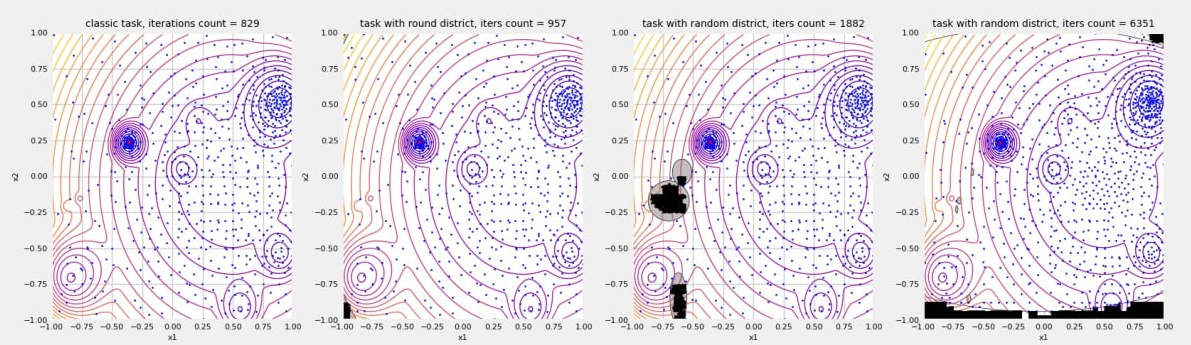
\includegraphics[width=450pt]{pic/fig_2.jpg}
\caption{Распределение точек испытаний при решении задач с различными невычислимыми областями} \label{fig_2}
\end{figure}

\subsection{Сравнение с другими алгоритмами}

...

\section{Заключение}

В данной работе была рассмотрена задача нахождения глобального минимума дорогостоящей липшицевой функции вида ``черный ящик''. По сравнению с традиционной формулировкой, используемой в глобальной оптимизации, задача рассмотренная здесь имеет важное отличие: целевая функция может быть не определена в некоторых подобластях области поиска (в частном случае, в одной или нескольких ее точках). В таких подобластях невозможно корректно провести численное моделирование и вычислить значение целевой функции.

Основная трудность заключается в невозможности в большинстве случаев заранее узнать о подобластях невычислимости, фактически, область допустимых сочетаний параметров является заранее неопределенной. Данное явление можно интерпретировать либо как наличие в задаче некоторых скрытых ограничений.

В статье было приведено описание одной из исследованных ранее модификаций алгоритма глобального поиска для решения такого класса задач. Приведены теоретические обоснования сходимости алгоритма. Теоретические результаты полностью соответсвуют картине, полученой в ходе экспериментальных исследований эффективности алгоритма. Разработанная модификация обладает недостатком в виде избыточных испытаний в области невычислимости (в силу порождения алгоритмом предельных точек в данных областях). Данного явления можно избежать с использованием более сложной модификации, восстанавливающей значения в невычислимых точках, основываясь на предположении о липшивости целевой функции (что было отражено в экспериментальных исследованиях). Теоретическое обоснование данной модификации является объектом будущих исследований.

%=======================  Список литературы ==================================
%
% Команда \LITERRUS печатает "СПИСОК ЛИТЕРАТУРЫ" и обнуляет счетчики
%
\LITERRUS
% \rlitem{arg1}{arg2} --- создает пункт списка литературы.
% arg1 --- символическая ссылка на источник, используется при создании ссылки командой \ref
% arg2 --- текст, помещаемый в пункт списка. Может содержать команды выбора начертания 
%          символов и др.

%7 - замена
\rlitem{rfa:rulit:Grishagin2016_2}{%
\textit{Grishagin~V.A., Israfilov~R.A., Sergeyev~Y.D.}
Convergence conditions and numerical comparison of global optimization methods based on dimensionality reduction schemes~// 
Appl. Math. Comput. 2018. \textbf{318}. 270--280.
\doi{10.1016/j.amc.2017.06.036}.
}
%9
\rlitem{rfa:rulit:Jones2021}{%
\textit{Jones~D., Martins~J.}
The direct algorithm: 25 years later~// 
J. Glob. Optim. 2021. \textbf{79}, N~3. 521--566.
\doi{10.1007/s10898-020-00952-6}.
}
%12
\rlitem{rfa:rulit:PaulaviciusZilinskas2014}{%
\textit{Paulavi{\v c}ius~R. and {\v Z}ilinskas~J.}
Simplicial Global Optimization.
New York: Springer, 2014.
\doi{10.1007/978-1-4614-9093-7}.
}
%13
\rlitem{rfa:rulit:Birect2020}{%
\textit{Paulavi{\v c}ius~R., Sergeyev~Y.D., Kvasov~D.E., {\v Z}ilinskas~J.}
Globally-biased {BIRECT} algorithm with local accelerators for expensive global optimization~// 
Expert Syst. Appl. 2020. \textbf{144}. 113052.
\doi{10.1016/j.eswa.2019.113052}.
}
%14  - замена на русскую
 \rlitem{rfa:rulit:Sergeyev2017}{%
\textit{Сергеев~Я.Д., Квасов~Д.Е.}
Диагональные методы глобальной оптимизации.
М.: Физматлит, 2008.
}
%11 - замена
\rlitem{rfa:rulit:Sovrasov2019}{%
\textit{Sovrasov~V.}
Comparison of several stochastic and deterministic derivative-free global optimization algorithms~// 
Lecture notes in computer science. 2019. \textbf{11548}. 70--81.
}
%15
\rlitem{rfa:rulit:Sergeyev2018}{%
\textit{Sergeyev~Y.D., Kvasov~D.E., Mukhametzhanov~M.S.}
On the efficiency of nature-inspired metaheuristics in expensive global optimization with limited budget~// 
Sci. Rep. 2018. \textbf{8}, N~1. 435.
}
%16
\rlitem{rfa:rulit:Sergeyev2013}{%
\textit{Sergeyev~Y.D., Strongin~R.G., Lera~D.}
Introduction to Global Optimization Exploiting Space-Filling Curves.
New York: Springer Briefs in Optimization, 2013.
\doi{10.1007/978-1-4614-8042-6}.
}
%20
\rlitem{rfa:rulit:Strongin2000}{%
\textit{Strongin~R.G., Sergeyev~Y.D.}
Global optimization with non-convex constraints. Sequential and parallel algorithms.
Dordrecht: Kluwer Academic Publishers, 2000.
}
%10 - замена на русскую
\rlitem{rfa:rulit:Kvasov2013}{%
\textit{Квасов~Д.Е., Сергеев~Я.Д.}
Методы липшицевой глобальной оптимизации в задачах управления~// 
Автоматика и телемеханика. 2013. №~9. 3--19.
}
%17
\rlitem{rfa:rulit:Sergeyev2020}{%
\textit{Sergeyev~Y.D., Candelieri~A., Kvasov~D.E., Perego~R.}
Safe global optimization of expensive noisy black-box functions in the $\delta$-Lipschitz framework~// 
Soft Comput. 2020. \textbf{24}, N~23. 17715--17735.
\doi{10.1007/s00500-020-05030-3}.
}
%Новая статья
\rlitem{rfa:rulit:Modorskii}{%
\textit{Калюлин~С.Л., Саженков~Н.А., Модорский~В.Я., Владимиров~Н.В.}
Численное моделирование газодинамических и прочностных характеристик вентилятора для экспериментальной установки по исследованию разрушения льда на вращающихся рабочих лопатках ~// 
Вестник Пермского национального исследовательского политехнического университета. Механика. 2023. №~1. 134--141.
\doi{10.14529/jsfi200101}.
}


%4 - убрать
\rlitem{rfa:rulit:Dongarra2022}{%
\textit{Dongarra~J.J.}
The evolution of mathematical software~// 
Commun. ACM. 2022. \textbf{65}, N~12. 66--72.
\doi{10.1145/3554977}.
}
%5 - убрать
\rlitem{rfa:rulit:Duwe2020}{%
\textit{Duwe~K., et al.}
State of the art and future trends in data reduction for high-performance computing~// 
Supercomput. Front. Innov. 2020. \textbf{7}, N~1.
\doi{10.14529/jsfi200101}.
}
%19
\rlitem{rfa:rulit:Stripinis2021}{%
\textit{Stripinis~L., Paulavi{\v c}ius~R.}
A new {DIRECT}-{GLh} algorithm for global optimization with hidden constraints~// 
Optim. Lett. 2021. \textbf{15}, N~6. 1865--1884.
\doi{10.1007/s11590-021-01726-z}.
}
%1
\rlitem{rfa:rulit:Audet2022}{%
\textit{Audet~C., Batailly~A., Kojtych~S.}
Escaping unknown discontinuous regions in blackbox optimization~// 
SIAM J. Optim. 2022. \textbf{32}, N~3. 1843--1870.
\doi{10.1137/21m1420915}.
}
%3
\rlitem{rfa:rulit:Candelieri2019}{%
\textit{Candelieri~A.}
Sequential model based optimization of partially defined functions
under unknown constraints~// 
J. Glob. Optim. 2019. \textbf{79}, N~2. 281--303.
\doi{10.1007/s10898-019-00860-4}.
}
%18 - убрать
\rlitem{rfa:rulit:Sergeyev2003}{%
\textit{Sergeyev~Y.D., Pugliese~P., Famularo~D.}
Index information algorithm with local tuning for solving multidimensional global optimization problems with multiextremal constraints~// 
Math. Program. 2003. \textbf{96}, N~23. 489--512.
\doi{10.1007/s10107-003-0372-z}.
}
%21
\rlitem{rfa:rulit:Strongin2020}{%
\textit{Strongin~R.G., Barkalov~K.A., Bevzuk~S.A.}
Global optimization method with dual Lipschitz constant estimates for problems with non-convex constraints~// 
Soft Comput. 2020. \textbf{24}, N~16. 11853--11865.
\doi{10.1007/s00500-020-05078-1}.
}

\rlitem{rfa:rulit:Usova2024}{%
\textit{M.~A.~Usova, K.~A.~Barkalov} 
An Algorithm for Finding the Global Extremum of a Partially Defined Function~// Communications in Computer and Information Science. 2024. {\bf 1914}. 147--161.
\doi{10.1007/978-3-031-52470-7_13}.
}
%2
\rlitem{rfa:rulit:Barkalov2022}{%
\textit{Barkalov~K.A., et al.}
On solving the problem of finding kinetic parameters of catalytic isomerization of the pentane-hexane fraction using a parallel global search algorithm~// 
Mathematics. 2022. \textbf{10}, N~19. 3665.
\doi{10.3390/math10193665}.
}
%8
\rlitem{rfa:rulit:Gubaydullin2022}{%
\textit{Gubaydullin~I.M., Enikeeva~L.V., Barkalov~K.A., Lebedev~I.G., Silenko~D.G.}
Kinetic modeling of isobutane alkylation with mixed c4 olefins and sulfuric acid as a catalyst using the asynchronous global optimization algorithm~// 
Commun. Comput. Inf. Sci. 2022. \textbf{1618}. 293--306.
\doi{10.1007/978-3-031-11623-0_20}.
}
%6
\rlitem{rfa:rulit:Gaviano2003}{%
\textit{Gaviano~M., Kvasov~D.E., Lera~D., Sergeyev~Y.D.}
Software for generation of classes of test functions with known local and global minima for global optimization~// 
ACM Trans. Math. Softw. 2003. \textbf{29}, N~4. 469--480.
}

%=======================  Список литературы ==================================
\medskip
\DateRU 

\medskip

\MakeAuthorsInfoRU

%===========================  REFERENCES =====================================
\pagebreak

\REFERENCES

%7
\elitem{rfa:enlit:Grishagin2016_2}{%
V.~A.~Grishagin, R.~A.~Israfilov, ``Global search acceleration in the nested optimization scheme'',
AIP Conference Proceedings. {\bf 1738}, 400010 (2016). 
\doi{10.1063/1.4952198}.
}
%9
\elitem{rfa:enlit:Jones2021}{%
D.~Jones, J.~Martins, ``The direct algorithm: 25 years later'',
J. Glob. Optim. {\bf 79} (3), 521--566 (2021). 
\doi{10.1007/s10898-020-00952-6}.
}
%12
\elitem{rfa:enlit:PaulaviciusZilinskas2014}{%
R.~Paulavi{\v c}ius and J.~{\v Z}ilinskas
{\it Simplicial Global Optimization}
(Springer, New York, 2014).
\doi{10.1007/978-1-4614-9093-7}.
}
%13
\elitem{rfa:enlit:Birect2020}{%
R.~Paulavi{\v c}ius, Y.~D.~Sergeyev, D.~E.~Kvasov, J.~{\v Z}ilinskas, ``Globally-biased {BIRECT} algorithm with local accelerators for expensive global optimization'', 
Expert Syst. Appl. {\bf 144}, 113052 (2020).
\doi{10.1016/j.eswa.2019.113052}.
}
%14
\elitem{rfa:enlit:Sergeyev2017}{%
Y.~D.~Sergeyev, D.~E.~Kvasov
{\it Deterministic global optimization: An introduction to the diagonal approach}
(Springer, New York, 2017).
\doi{10.1007/978-1-4939-7199-2}.
}
%11
\elitem{rfa:enlit:Liberti2005}{%
L.~Liberti, S.~Kucherenko, ``Comparison of deterministic and stochastic approaches to global optimization'',
Int. Trans. Oper. Res. {\bf 12}, 263--285 (2005).
}
%15
\elitem{rfa:enlit:Sergeyev2018}{%
Y.~D.~Sergeyev, D.~E.~Kvasov, M.~S.~Mukhametzhanov, ``On the efficiency of nature-inspired metaheuristics in expensive global optimization with limited budget'',
Sci. Rep. {\bf 8} (1), 435 (2018).
}
%16
\elitem{rfa:enlit:Sergeyev2013}{%
Y.~D.~Sergeyev, R.~G.~Strongin, D.~Lera
{\it Introduction to Global Optimization Exploiting Space-Filling Curves}
(Springer Briefs in Optimization, Springer, New York, 2013).
\doi{10.1007/978-1-4614-8042-6}.
}
%20
\elitem{rfa:enlit:Strongin2000}{%
R.~G.~Strongin, Y.~D.~Sergeyev
{\it Global optimization with non-convex constraints. Sequential and parallel algorithms}
(Kluwer Academic Publishers, Dordrecht, 2000).
}
%10
\elitem{rfa:enlit:Kvasov2013}{%
D.~E.~Kvasov, Y.~D.~Sergeyev, ``Lipschitz global optimization methods in control problems'',
Autom. Remote Control. {\bf 74} (9), 1435--1448 (2013).
\doi{10.1134/s0005117913090014}.
}
%17
\elitem{rfa:enlit:Sergeyev2020}{%
Y.~D.~Sergeyev, A.~Candelieri, D.~E.~Kvasov, R.~Perego, ``Safe global optimization of expensive noisy black-box functions in the $\delta$-Lipschitz framework'',
Soft Comput. {\bf 24} (23), 17715--17735 (2020).
\doi{10.1007/s00500-020-05030-3}.
}
%4
\elitem{rfa:enlit:Dongarra2022}{%
J.~J.~Dongarra, ``The evolution of mathematical software'', 
Commun. ACM. {\bf 65} (12), 66--72 (2022).
\doi{10.1145/3554977}.
}
%5
\elitem{rfa:enlit:Duwe2020}{%
K.~Duwe, et al., ``State of the art and future trends in data reduction for high-performance computing'',
Supercomput. Front. Innov. {\bf 7} (1), (2020).
\doi{10.14529/jsfi200101}.
}
%19
\elitem{rfa:enlit:Stripinis2021}{%
L.~Stripinis, R.~Paulavi{\v c}ius, ``A new {DIRECT}-{GLh} algorithm for global optimization with hidden constraints'',
Optim. Lett. {\bf 15} (6), 1865--1884 (2021).
\doi{10.1007/s11590-021-01726-z}.
}
%1
\elitem{rfa:enlit:Audet2022}{%
Audet~C., Batailly~A., Kojtych~S., ``Escaping unknown discontinuous regions in blackbox optimization'',
SIAM J. Optim. {\bf 32} (3), 1843--1870 (2022).
\doi{10.1137/21m1420915}.
}
%3
\elitem{rfa:enlit:Candelieri2019}{%
A.~Candelieri, ``Sequential model based optimization of partially defined functions under unknown constraints'',
J. Glob. Optim. {\bf 79} (2), 281--303 (2019).
\doi{10.1007/s10898-019-00860-4}.
}
%18
\elitem{rfa:enlit:Sergeyev2003}{%
Y.~D.~Sergeyev, P.~Pugliese, D.~Famularo, ``Index information algorithm with local tuning for solving multidimensional global optimization problems with multiextremal constraints'', 
Math. Program. {\bf 96} (23), 489--512 (2003).
\doi{10.1007/s10107-003-0372-z}.
}
%21
\elitem{rfa:enlit:Strongin2020}{%
R.~G.~Strongin, K.~A.~Barkalov, S.~A.~Bevzuk, ``Global optimization method with dual Lipschitz constant estimates for problems with non-convex constraints'',
Soft Comput. {\bf 24} (16), 11853--11865 (2020).
\doi{10.1007/s00500-020-05078-1}.
}

\elitem{rfa:enlit:Usova2024}{%
M.~A.~Usova, K.~A.~Barkalov, ``An Algorithm for Finding the Global Extremum of a Partially Defined Function'', Communications in Computer and Information Science. {\bf 1914}, 147--161 (2024).
\doi{10.1007/978-3-031-52470-7_13}.
}

%2
\elitem{rfa:enlit:Barkalov2022}{%
K.~A.~Barkalov, et al., ``On solving the problem of finding kinetic parameters of catalytic isomerization of the pentane-hexane fraction using a parallel global search algorithm'',
Mathematics. {\bf 10} (19), 3665 (2022).
\doi{10.3390/math10193665}.
}
%8
\elitem{rfa:enlit:Gubaydullin2022}{%
I.~M.~Gubaydullin, L.~V.~Enikeeva, K.~A.~Barkalov, I.~G.~Lebedev, D.~G.~Silenko, ``Kinetic modeling of isobutane alkylation with mixed c4 olefins and sulfuric acid as a catalyst using the asynchronous global optimization algorithm'',
Commun. Comput. Inf. Sci. {\bf 1618}, 293--306 (2022).
\doi{10.1007/978-3-031-11623-0_20}
}
%6
\elitem{rfa:enlit:Gaviano2003}{%
M.~Gaviano, D.~E.~Kvasov, D.~Lera, Y.~D.~Sergeyev, ``Software for generation of classes of test functions with known local and global minima for global optimization'',
ACM Trans. Math. Softw. {\bf 29} (4), 469--480 (2003).
}

\medskip
\DateEN

\bigskip

\MakeAuthorsInfoEN

%\end{document}
%============================ КОНЕЦ СТАТЬИ ==================================


%%%%%%%% В КОНЦЕ УДАЛИТЬ

%\section{Рекомендации к содержанию и структуре статей}

%Авторам оригинальных статей рекомендуется объем до 20 страниц.

%Объем аннотации не должен превышать 10--15 строк. Разбивать аннотации на абзацы не рекомендуется.

%Авторы статьи указывают УДК (для статей на русском языке), которым соответствует публикация.

%Рекомендуется для лучшего восприятия разбивать текст на абзацы размером не более 10--15~строк.

%Список литературы является неотъемлемой частью статьи и оформляется непосредственно в тексте статьи: использование отдельных файлов с расширениями bib, bbl и других не допускается. 

%Авторы статей, публикуемых в журнале на русском языке, должны предоставить переведенные на английский язык:
%\begin{itemize}[itemsep=0pt,parsep=0pt,topsep=0pt,partopsep=0pt]
%\item фамилию, имя, отчество, ученую степень, ученое звание и должность каждого автора;
%\item название, почтовые адреса организаций, являющихся основными местами работы авторов, и их должности в этих организациях;
%\item название статьи;
%\item текст аннотации;
%\item ключевые слова;
%\item слова благодарности;
%\item подписи к рисункам, таблицам, листингам программ и алгоритмов, а также всю текстовую информацию, содержащуюся на рисунках, в таблицах и пр.
%\end{itemize}
%\vspace*{2mm}


%Между инициалами и фамилией всегда должен ставится пробел (А.А.~Иванов).
%В заголовке статьи пробелы также ставятся между инициалами: А.~А.~Иванов.

%Точка не ставится после заголовков разделов, названий таблиц и подписей рисунков, после ряда сокращенных наименований: с~--- секунда, г~--- грамм, мин~--- минута, сут~--- сутки, млн~--- миллион, млрд~--- миллиард и т.п. Точка ставится в конце последнего предложения аннотации, в конце списка ключевых слов, после сокращений: мес.~--- месяц, г.~--- год и др.

%Для набора выключных формул рекомендуется использовать окружение {\tt equation} с автоматической сквозной нумерацией. Для подавления нумерации используйте окружение {\tt equation*}.

%\pagebreak
%\smallskip

%\item Слова ``Теорема'', ``Следствие'', ``Лемма'', ``Утверждение'', ``Предложение'' помещаются в текст статьи явно и выделяются прямым полужирным шрифтом, а соответствующие формулировки печатаются прямым шрифтом.
%\item Слова ``Доказательство'', ``Определение'', ``Примечание'', ``Замечание'' выделяются прямым полужирным шрифтом, а соответствующие формулировки печатаются прямым шрифтом.
%\item Рекомендуется выполнять сквозную нумерацию арабскими цифрами для теорем, %лемм, определений и т.д. 

%Допускается воспроизводить небольшие по объему (рекомендуется не более 1 страницы) фрагменты программ, иллюстрирующие важные для понимания статьи алгоритмы, средства языков программирования и т.п. Текстовые сообщения и комментарии в листингах должны быть представлены на английском языке.

%Рекомендуются следующие размеры иллюстраций: а)~шириной не более 165~мм и высотой не более 210~мм (в ширину колонки текста); б)~шириной не более 80 мм и высотой не более 140~мм (в половину ширины колонки); в) высотой 145~мм и шириной 240~мм (иллюстрация, развернутая на $90^\circ$ на всю страницу).
%Принимаются иллюстрации трех видов: штриховые рисунки (графики, диаграммы, графы и пр.), скриншоты экрана компьютера (например, цветовая визуализация поля, полученная в результате математического моделирования) и фотографии.
%Штриховые рисунки принимаются в виде файлов формата PNG (растр) разрешением 600 DPI при масштабе рисунка 1:1 или в формате EPS (векторные рисунки). Толщина самой тонкой линии на рисунке не должна быть меньше 5~px. Рекомендуется для основных линий использовать черный цвет. Важные для понимания элементы рисунка должны выделяться двумя-тремя цветами, которые контрастно воспроизводятся при черно-белой печати. Цвет фона рекомендуется белый. Фотографии принимаются в форматах JPEG, PNG, TIFF разрешением 300 DPI. Изображение на фотографии должно быть резким, контрастным. Цифровая обработка изображения не должна вызывать сомнений в достоверности фотографии. Надписи на рисунках должны быть выполнены на английском языке. Рекомендуется важные элементы рисунка обозначать цифрами и давать расшифровку в подписи. Серия иллюстраций предназначается для сравнения графиков, оценки влияния параметров, объяснения трендов, динамики и т.п. Рисунки, входящие в серию, должны быть одинакового размера и разрешения. Каждая иллюстрация в серии должна быть обозначена буквой английского алфавита.
%Редакция просит предоставлять наряду с файлами EPS исходные, необработанные файлы в форматах TIFF, PNG, JPEG. 
    
%Подписи к рисункам, заголовки таблиц, листингов программ и алгоритмов должны быть выполнены на русском и английском языках. Для этого в стилевом файле определены команды \verb!\bicaption!.

%Список литературы формируется в порядке обращения к источникам в       тексте статьи.

%Для уменьшения вероятности ошибок в ссылках по тексту статьи необходимо пользоваться командами \verb!\label!, автоматически сохраняющей значения счетчиков для рисунков, таблиц, списков в символической переменной, и \verb!\ref!, которая создает ссылку по имени переменной.

%Необходимые документы
%Для публикации статьи авторы должны предоставить: 
% сопроводительное письмо авторов (Приложение~1 в этом документе) в электронном виде и его отсканированный вариант с ``живыми'' подписями;
% электронную \LaTeX--версию статьи (на русском или/и английском языках), подготовленную в соответствии с требованиями к оформлению статей, а также pdf--файл статьи и рисунки;
% текстовый файл, содержащий следующую информацию на русском и английском языках: а)~фамилия, имя, отчество, ученая степень, ученое звание, ORCID и e-mail каждого из авторов; б)~названия и почтовые адреса организаций, являющихся основными местами работы авторов и их должности в этих организациях; в)~название статьи; г)~текст аннотации; д)~ключевые слова.
%Автор взаимодействует с редакцией в основном через сайт журнала \url{https://num-meth.ru}. После заполнения регистрационной формы автор (один из авторов) должен:
%\item загрузить через форму все подготовленные необходимые документы и компоненты статьи в виде ZIP--архива, выбрав при загрузке {\tt Компонент статьи = ``ZIP-архив с исходными текстами (.tex и требуемые дополнительные файлы)''};
%\item дать описание архива, авторство и т.п. (рекомендуется сделать на этапе проверки деталей отправляемого файла);
%\item подтвердить отправку архива;
%\item ввести метаданные статьи (обязательно заголовок, аннотацию и ключевые слова) и информацию об авторе и всех соавторах (вся информация должна заноситься на русском и дублироваться на английском языке);
%\item подтвердить внесенные данные.

%%%%%%%% В КОНЦЕ УДАЛИТЬ

%============================ ПРИЛОЖЕНИЕ 6 ==================================
\newpage\nolinenumbers
%
% ПРИЛОЖЕНИЕ 4
% используйте как шаблон письма в редакцию
%
\thispagestyle{empty}
%
% Следующие две строки нужно убрать
%
%\appendix{Сопроводительное письмо в редакцию}{pril:sopr}
%

{\large
\hfill\parbox[t]{80mm}{
Главному редактору научного журнала\\[2mm]
``Вычислительные методы и\\
программирование''\\[2mm]
чл.-корр. РАН, проф. Вл. В. Воеводину
}
\vspace*{12mm}
\begin{center}
СОПРОВОДИТЕЛЬНОЕ ПИСЬМО
\end{center}

\vspace*{3mm}

Просим опубликовать в журнале ``Вычислительные методы и программирование'' статью 
``<НАЗВАНИЕ СТАТЬИ>''.

Сообщаем следующую информацию о каждом авторе статьи.

1. Фамилия, имя, отчество полностью (с написанием на английском языке).

2. Основное место работы полностью с указанием полного почтового адреса и URL сайта организации (с переводом на английский язык).

3. Должность по основному месту работы (с переводом на английский язык).

4. Ученая степень и ученое звание (с переводом на английский язык).

5. Телефон служебный, домашний и мобильный.

6. E-mail.

7. ORCID (\corr{обязательно}; если еще не получен, посетите \url{https://orcid.org/register}).

8. Номер и название рубрики ГРНТИ (только для статей на русском) и код OECD для подаваемой статьи.

9. Желательно: ссылки на профили авторов в elibrary.ru для упрощения и корректности подлинковки статьи.

\vspace*{2mm}
Текущую переписку по вопросам публикации статьи следует вести с <Фамилия И.О.>.

\vspace*{2mm}
Авторы согласны с правилами подготовки статьи к публикации, включая рецензирование, 
научное и литературное редактирование и доведение статьи до редакторских стандартов, 
принятых в рамках журнала.

Авторы ознакомлены с Публикационной этикой журнала и согласны с ее положениями.

Авторы также согласны с передачей журналу своего права на издание и распространение 
статьи в электронной и бумажной версиях, в том числе на размещение библиографической 
информации о статье в Российском индексе научного цитирования (РИНЦ) и в других базах 
научного цитирования и на размещение полных текстов статей в Научной электронной 
библиотеке (elibrary.ru) и портале http://www.mathnet.ru для свободного доступа всем пользователям Интернет независимо от их категории и местоположения.

\vspace*{15mm}
<Дата>\hfill\parbox[t]{70mm}{\hrulefill~<И.О. Фамилия>}

\vspace*{8mm}

\hfill\parbox[t]{70mm}{\hrulefill~<И.О. Фамилия>}

}%large

\end{document}

